\subsection{HR} 
\label{HR_manual}
%Maike and Philipp
One of the most critical resources that a company needs in order to get a competitive advantage, are the human resources (HR).
The goal of the HR department is to maximize the employee performance in order to support the vision of the company. The HR department has many responsibilities. This includes personnel planning, recruitment, compensation and benefits, training and development and performance management.

%what is meant by time / duration?
Personnel planning contains the determination of employee requirements, including number (capacity per head), quality, time / duration, location (domestic / foreign, location, department, cost center) and costs. Steps of recruitment are needs assessment, advertising, selection, negotiation and introduction / training. The aim is to achieve a cost-effective and fast procurement of the desired employees, which involves identifying and hiring high-performing employees. 

Compensation and benefits means creating, managing and improving a company's compensation and performance structures. Wages and benefits are two crucial factors that ultimately determine how well your employees feel about your company and how likely they are to stay with it in the future.

Training and development includes the ability to create training programs that solve the performance problems of employees and create additional incentives for employees to improve further and thus also advance the company.

Furthermore, the development and implementation of a complete performance management and improvement process is an essential capability of a company. The design of the performance assessment process, its maintenance and the effective monitoring of its implementation represent challenging tasks for a company. 

As not all of the above mentioned tasks are suitable for a simulation game, we concentrated on some aspects which are of strategic importance.

The HR process of the CapX Game is mainly structured in three phases
\begin{enumerate}
    \item Hiring
    \item Development
    \item Motivation
\end{enumerate}

For CapX there are two types of employees of main importance: engineers and sales employees. In order to be able to produce products it is necessary to hire available engineers on the market. Moreover, to sell the produced products, sales people are needed who are responsible for the entire sales cycle of the company.

\begin{figure} [!htbp]
    \centering
    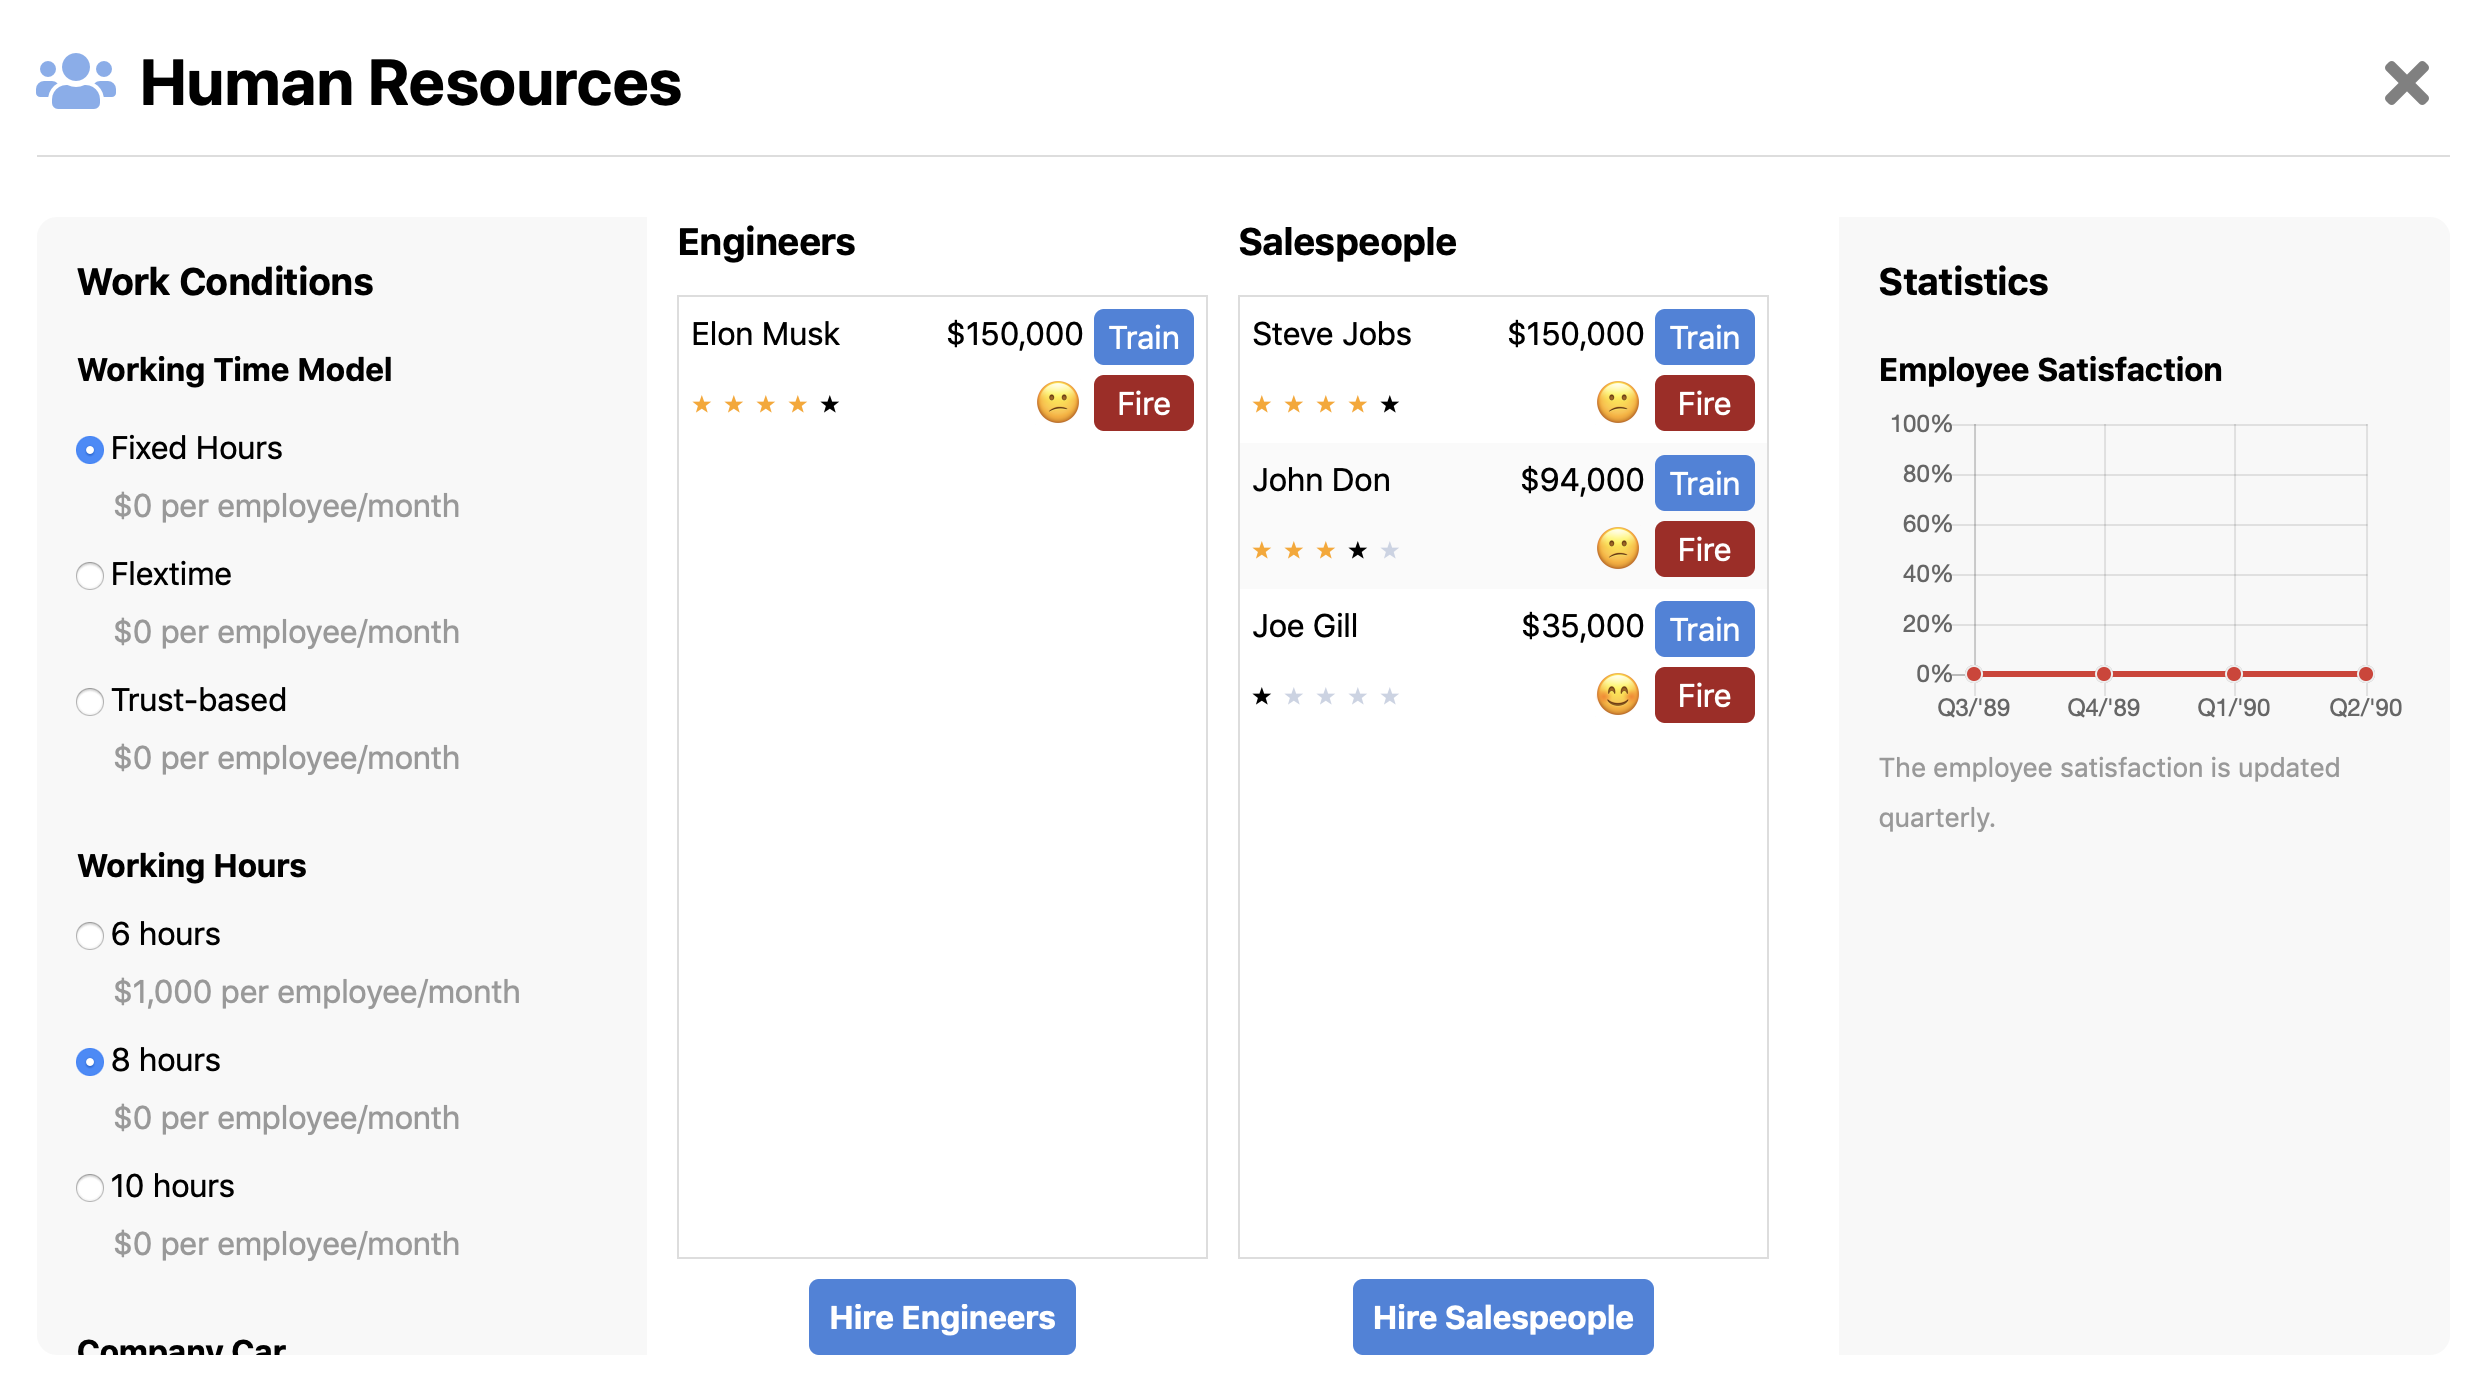
\includegraphics [width=\textwidth]{HR/hr_view.png}
    \caption{Navigation Bar}
    \label{fig:navigationBar}
\end{figure}

The HR view allows you to see the available employees on the market per department. For each employee you will see their names, their skilllevel (indicated by stars) and their salary demand. Depending on your own HR strategy you will have to decide whom to hire. Be advised that hiring and firing employees is not a one time activity but rather a constant task. Your strategy needs to be executed throughout the entire game.

After you made your initial first decision about your workforce you can start the workforce development by choosing the necessary training for your employees. In order to develop, grow and gain new knowledge, your employees are required to be trained continuously. Lifelong learning is an essential part of every HR strategy. By clicking the train button you can train single employees, but also entire teams. Make sure that you really choose a training that fits to the needs of your employees so that they can maximize their benefit from it.

The third pillar of your HR strategy is the motivation. Providing the right extrinsic motivation is necessary, so that your employees feel valued. The extrinsic motivation can be provided through the usage of benefits. On the one hand, benefits motivate employees and ensures a positive contribution to the work-life-balance, but on the other hand, of course, benefits cost money. Your task is to find the best possible balance and especially execute on your strategy. Make sure to think first, which HR strategy you have and then choose your options wisely. The benefits view is also provided in your HR view.